\section{Langkah-langkah Percobaan}

\subsection{Percobaan 1 (Judul)}
\begin{enumerate}
	\item Nyalakan Mikrotik
	\begin{figure}[H]
		\centering
		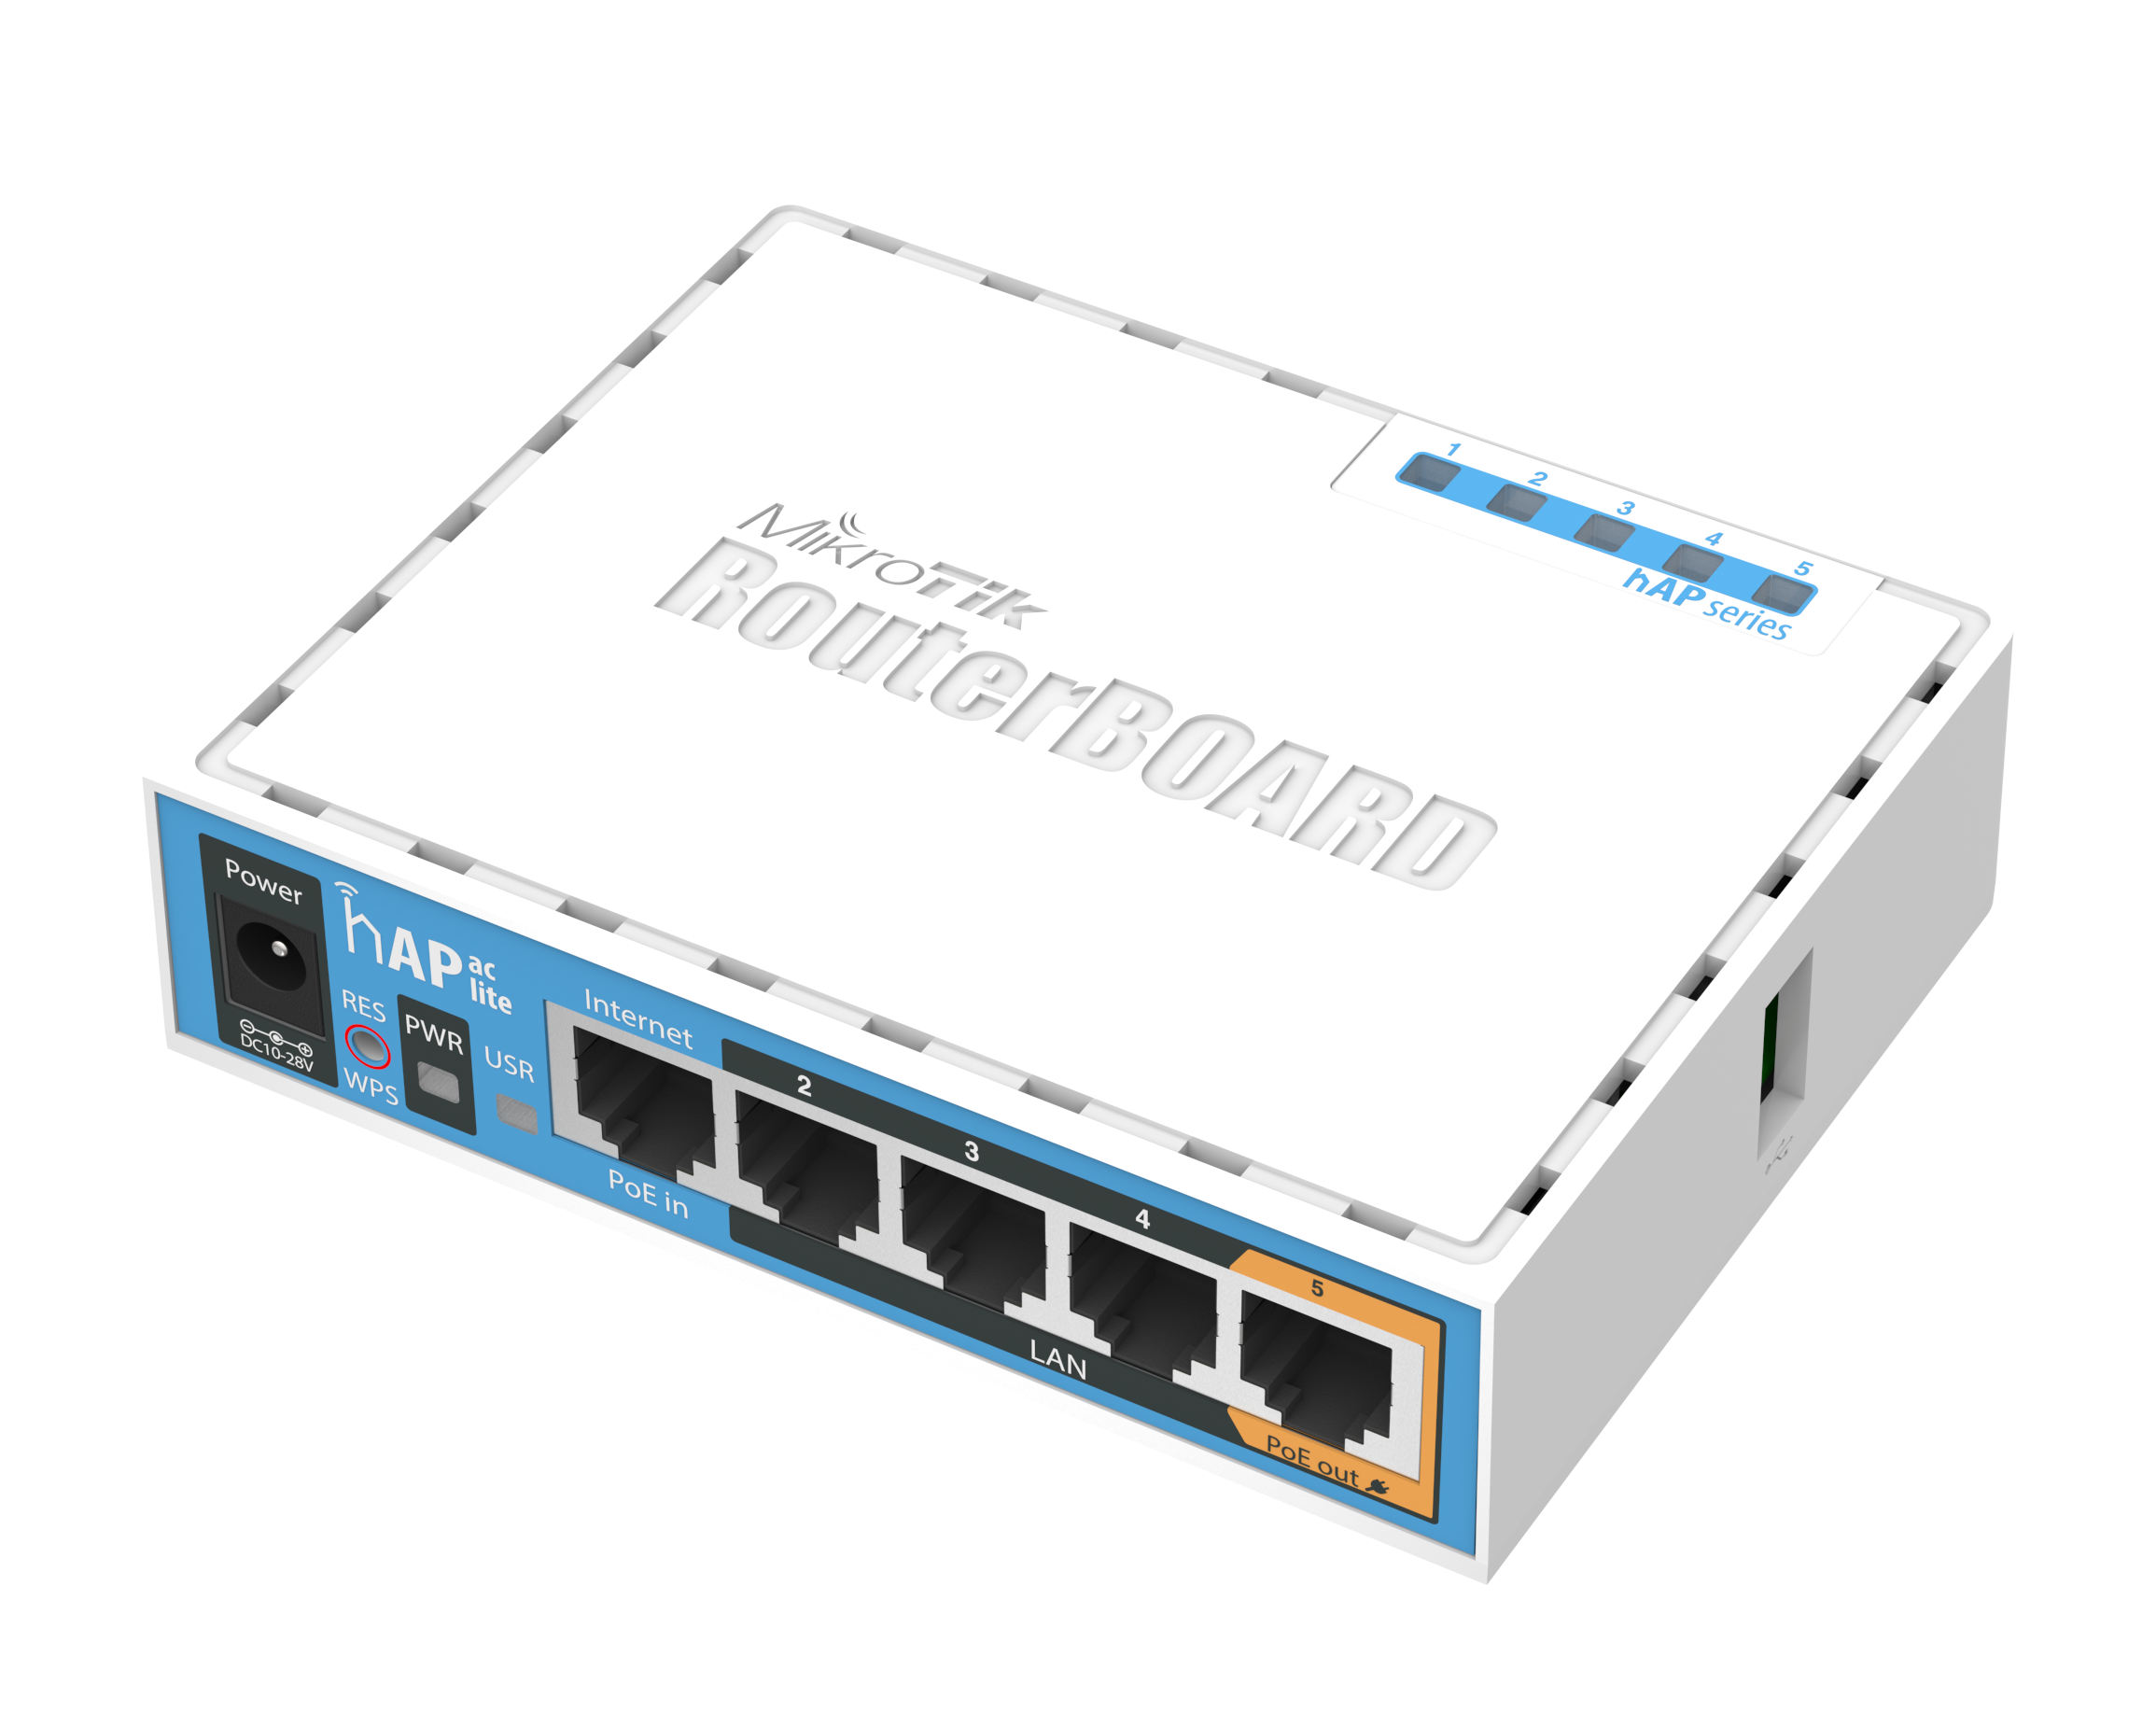
\includegraphics[width=0.5\linewidth]{P1/img/Mikrotik.png}
		\caption{Gambar Contoh}
		\label{fig:gambar1}
	\end{figure}
\end{enumerate}

\subsection{Percobaan 2 (Judul)}
\begin{enumerate}
	\item 
\end{enumerate}
%===========================================================%
\section{Analisis Hasil Percobaan}
 Hasil dari percobaan: apa yang terjadi saat percobaan, apa yang berjalan/bermasalah, dan penjelasan kenapa.
%===========================================================%
\section{Hasil Tugas}
 Hasil tugas modul yang dikerjakan setelah selesai praktikum.
%===========================================================%
\section{Kesimpulan}
Hasil kesimpulan selama melakukan praktikum.
%===========================================================%
\section{Lampiran}
\subsection{Dokumentasi saat praktikum}
\subsection{Hasil Challenge Modul}
